\chapter{Bilinear Maps}

We introduce Bilinear Maps and two of its applications: NIKE, Non-Interactive Key Exchange; and IBE, Identity Based Encryption.


\section{Diffie-Hellman Key Exchange}

\begin{figure}[H]
\label{fig:dh}
\centering
  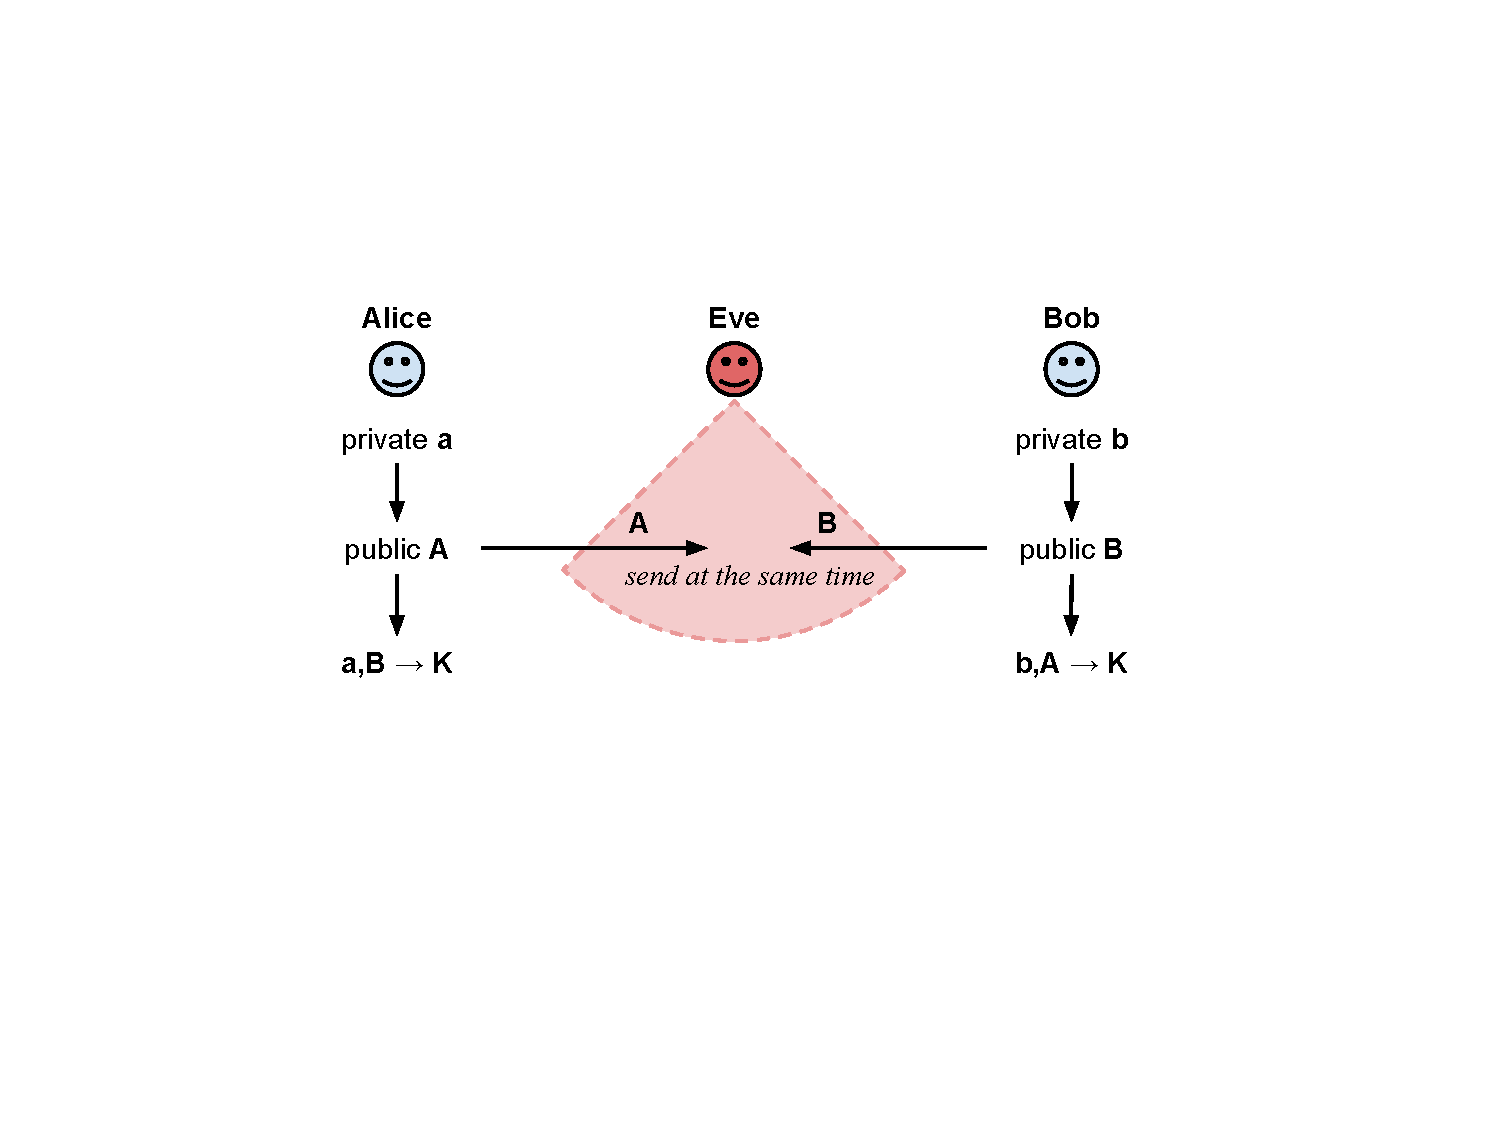
\includegraphics[width=0.7\textwidth]{fig1.pdf}
\caption{Diffie-Hellman Key Exchange}
\end{figure}


Fig \ref{fig:dh} illustrates Diffie-Hellman key exchange. Alice and Bob each has a private key ($a$ and $b$ respectively), and they want to build a shared key for symmetric encryption communication. They can only communicate over a insecure link, which is eavesdropped by Eve.
So Alice generates a public key $A$ and Bob generates a public key $B$, and they send their public key to each other at the same time. Then Alice generates the shared key $K$ from $a$ and $B$, and likewise, Bob generates the shared key $K$ from $b$ and $A$.
And we have $\forall$ PPT Eve, $Pr[k=Eve(A,B)]=neg(k)$, where $k$ is the length of $a$.


\subsection{Discussion 1}

Assume that $\forall (g, p)$, and $a_1,b_1 \stackrel{\$}{\gets} Z^*_p$, and $a_2,b_2,r \stackrel{\$}{\gets}Z^*_p$, we have $(g^{a_1}, g^{b_1}, g^{a_1b_1}) \stackrel{c}{\simeq} (g^{a_2}, g^{b_2}, g^r)$. How to apply this to Diffie-Hellman Key Exchange?


Make $A=g^a$, $B=g^b$, $K=A^b=g^{ab}$, and $K=B^a=g^{ab}$.


\subsection{Discussion 2}


How does Diffie-Hellman Key Exchange imply Public Key Encryption?


Alice
$pk = A$, $sk = a$, $Enc(pk, m \in \{0, 1\})$.

Bob
$b,r \gets Z^*_p$
$(g^b, mA^b+(1-m)g^r)$

Alice $Dec(sk, (c_1, c_2))$

$c_1^a \stackrel{?}{=} c_2$




\section{Bilinear Maps}

\begin{definition}{Bilinear Maps}

Bilinear Maps is $(G,P,G_T,g,e)$, where $e$ is an efficient function $G \times G \to G_T$ such that

\begin{itemize}
\item if $g$ is generator of $G$, then $e(g, g)$ is the generator of $G_T$.
\item $\forall a,b \in Z_p$, we have $e(g^a, g^b) = e(g, g)^{ab} = e(g^b, g^a)$.
\end{itemize}

\end{definition}

\subsection{Discussion 1}


How does Bilinear Maps apply to Diffie-Hellman?

Make $A=g^a$, $B=g^b$, and $T=g^{ab}$, then Diffie-Hellman has $e(A, B)=e(g, T)$.


\section{Tripartite Diffie-Hellman}

\begin{figure}[H]
\label{fig:3dh}
\centering
  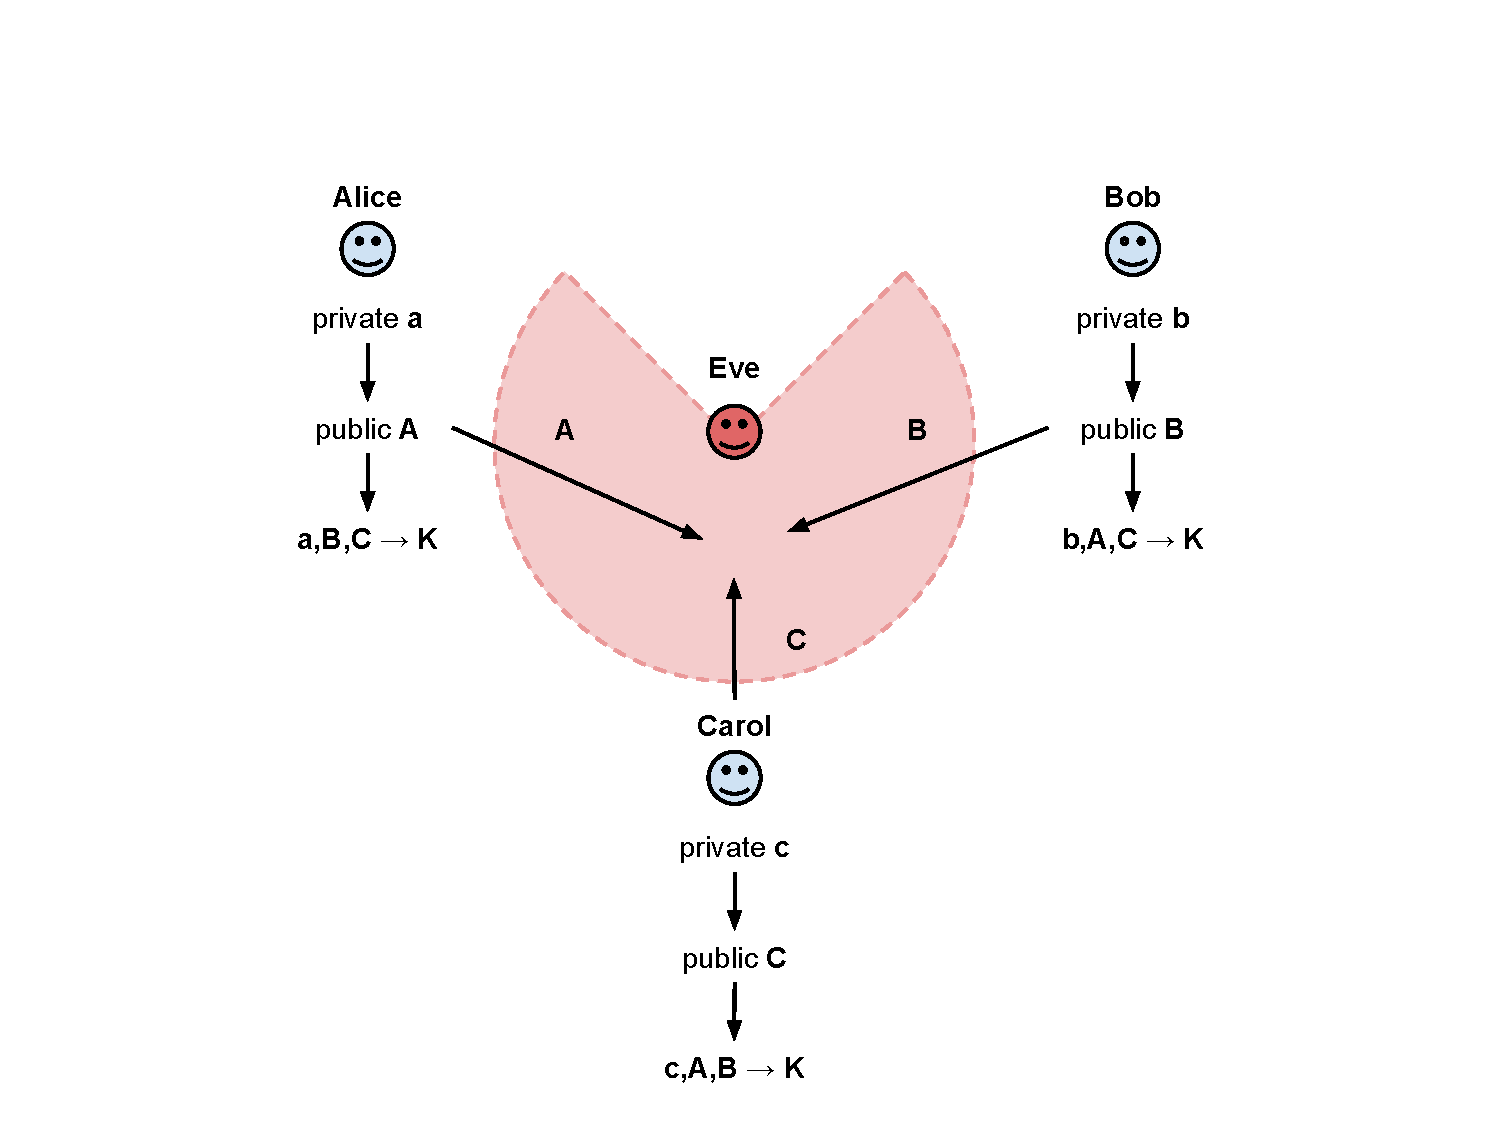
\includegraphics[width=0.7\textwidth]{fig2.pdf}
\caption{Tripartite Diffie-Hellman Key Exchange}
\end{figure}

Fig \ref{fig:3dh} illustrates Tripartite Diffie-Hellman key exchange. $a$, $b$, and $c$ are private key of Alice, Bob, and Carol, respectively.
They use $g^a$, $g^b$, $g^c$ as public key, and the shared key $K=e(g,g)^{abc}$.
Formally, we have
$$a,b,c \stackrel{\$}{\gets} Z^*_p, r \stackrel{\$}{\gets} Z^*_p$$
$$A=g^a, B=g^b, C=g^c$$
$$K=e(g,g)^{abc}$$



\section{IBE: Identity-Based Encryption}
IBE contains four steps: \emph{Setup}, \emph{KeyGen}, \emph{Enc}, and \emph{Dec}. We illustrate it in Figure \ref{fig:ibe}.
In first step, Key authority get a Master Public Key (MPK) and Master Signing Key (MSK) from $Setup(1^k)$. Then a user with an ID
 (in this example, ``Mike''), sends his ID to the key authority. The key authority generates the Signing Key of Mike with $KeyGen(MSK, ID)$ ans sends it back. Another use, Alice, wants to send an encrypted message to Mike. She only has MPK and Mike's ID. So she encrypts the message with $c=Enc(MPK, ID=Mike, m)$, and sends the encrypted message $c$ to Mike. Mike decodes $c$ with $m=Dec(c, SK_{Mike})$. Notice that Alice never need to know Mike's public key. She only needs to remember MPK and other people's IDs.

\begin{figure}[H]
\label{fig:ibe}
\centering
  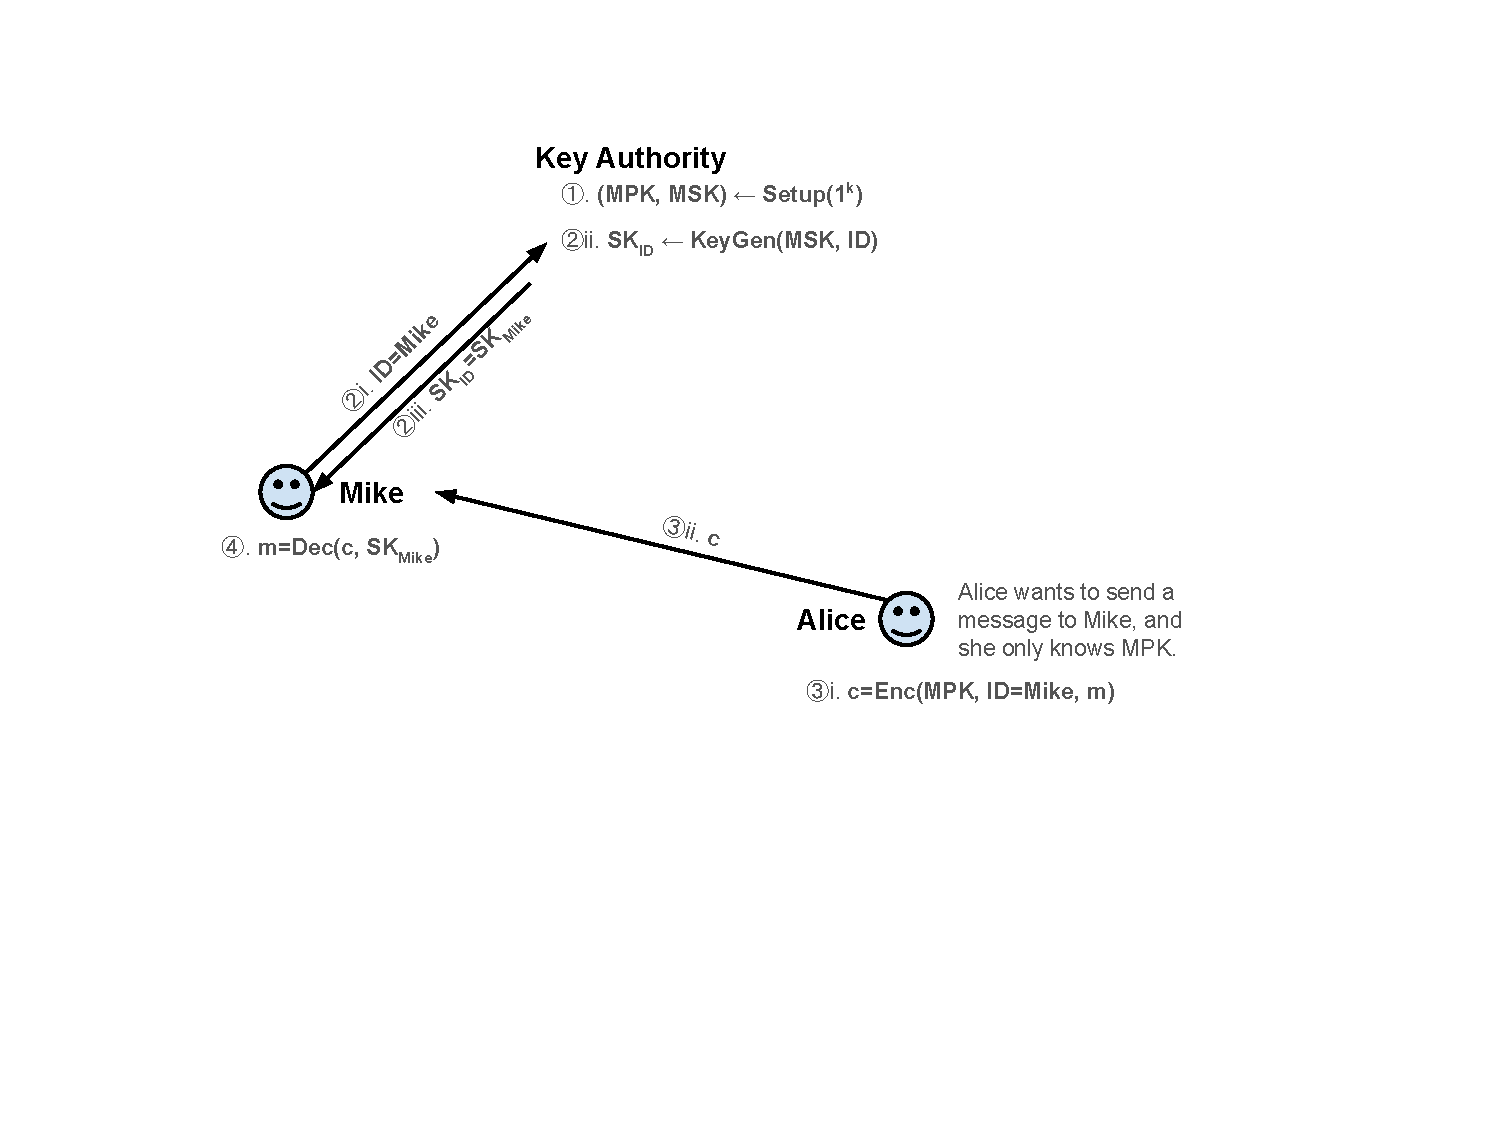
\includegraphics[width=0.7\textwidth]{fig3.pdf}
\caption{Identity-Based Encryption}
\end{figure}

Formally, we have

$$Pr\begin{bmatrix}
       (MPK, MSK) \gets Setup(1^k), \\[0.3em]
       SK_{ID} \gets KeyGen(MSK, ID), \\[0.3em]
       c \gets Enc(MPK, ID, m), \\[0.3em]
       m \gets Dec(SK_{ID}, c)
     \end{bmatrix}
      =1$$

\subsection{Security Descriptions}

We have different security descriptions for IBE, as discussed in this section.

\subsubsection{CCA1}
\begin{tabular}{ r c l }
  \textbf{Challenger} & & \textbf{Adversary} \\
  $(MPK, MSK) \gets Setup(1^k)$ & $\xrightarrow{MPK}$ &  \\
   & $\xleftarrow{ID_1}$ & \\
  $SK_{ID_1} \gets KeyGen(MSK, ID_1)$ & $\xrightarrow{SK_{ID_1}}$ & \\
  $\vdots$ & $\vdots$ & $\vdots$ \\
   & $\xleftarrow{ID_i}$ & \\
  $SK_{ID_i} \gets KeyGen(MSK, ID_i)$ & $\xrightarrow{SK_{ID_i}}$ & \\
   & $\xleftarrow{ID^*, m_0, m_1}$ & $\forall i \in [q], ID^* \neq ID_i$\\
  $b \overset{\$}{\gets} \{0, 1\}$, $c^* = Enc(MPK, ID^*, m_b)$ & $\xrightarrow{c^*}$ & \\
  Output $1$ if $b' = b$, otherwise $0$ & $\xleftarrow{b'}$ & \\
\end{tabular}

\subsubsection{CCA2}
In CCA2, we allow adversary to send further queries after getting $c^*$.

\begin{tabular}{ r c l }
  \textbf{Challenger} & & \textbf{Adversary} \\
  $(MPK, MSK) \gets Setup(1^k)$ & $\xrightarrow{MPK}$ &  \\
   & $\xleftarrow{ID_1}$ & \\
  $SK_{ID_1} \gets KeyGen(MSK, ID_1)$ & $\xrightarrow{SK_{ID_1}}$ & \\
   & $\vdots$ & \\
   & $\xleftarrow{ID_i}$ & \\
  $SK_{ID_q} \gets KeyGen(MSK, ID_q)$ & $\xrightarrow{SK_{ID_q}}$ & \\
   & $\xleftarrow{ID^*, m_0, m_1}$ & $\forall i \in [q'], ID^* \neq ID_i$\\
  $b \overset{\$}{\gets} \{0, 1\}$, $c^* = Enc(MPK, ID^*, m_b)$ & $\xrightarrow{c^*}$ & \\
   & $\xleftarrow{ID_{q+1}}$ & \\
  $SK_{ID_{q+1}} \gets KeyGen(MSK, ID_{q+1})$ & $\xrightarrow{SK_{ID_{q+1}}}$ & \\
  $\vdots$ & $\vdots$ & $\vdots$ \\
   & $\xleftarrow{ID_{q'}}$ & \\
  $SK_{ID_{q'}} \gets KeyGen(MSK, ID_{q'})$ & $\xrightarrow{SK_{ID_{q'}}}$ & \\
  Output $1$ if $b' = b$, otherwise $0$ & $\xleftarrow{b'}$ & \\
\end{tabular}

\subsubsection{Selective Security}
In selective security, the adversary sends $ID^*$ before everything.

\begin{tabular}{ r c l }
  \textbf{Challenger} & & \textbf{Adversary} \\
   & $\xleftarrow{ID^*}$ & $\forall i \in [q], ID^* \neq ID_i$\\
  $(MPK, MSK) \gets Setup(1^k)$ & $\xrightarrow{MPK}$ &  \\
   & $\xleftarrow{ID_1}$ & \\
  $SK_{ID_1} \gets KeyGen(MSK, ID_1)$ & $\xrightarrow{SK_{ID_1}}$ & \\
  $\vdots$ & $\vdots$ & $\vdots$ \\
   & $\xleftarrow{ID_q}$ & \\
  $SK_{ID_q} \gets KeyGen(MSK, ID_q)$ & $\xrightarrow{SK_{ID_q}}$ & \\
   & $\xleftarrow{m_0, m_1}$ & \\
  $b \overset{\$}{\gets} \{0, 1\}$, $c^* = Enc(MPK, ID^*, m_b)$ & $\xrightarrow{c^*}$ & \\
  Output $1$ if $b' = b$, otherwise $0$ & $\xleftarrow{b'}$ & \\
\end{tabular}


\subsection{Discussion 1}
How does Bilinear Maps apply to IBE?

Given Bilinear Maps: $(G, P, G_T, g, e)$, we have

\begin{enumerate}
\item $(G, P, G_T, g, e) \gets Setup(1^k)$
\item $s \gets Z^*_p$, and $H_1: \{0, 1\}^* \to G $, $H_2: G_T \to \{0, 1\}^n$
\item $MPK = (G, g^s, H_1, H_2)$, and $MSK = (s)$
\end{enumerate}

Let's look at how we construct each function in IBE.

\paragraph{$KeyGen(s, ID)$:}~\\
\begin{enumerate}
\item Output $SK_{ID} = (H_1(ID))^s$
\end{enumerate}

\paragraph{$Enc(MPK, ID, m)$:}~\\
\begin{enumerate}
\item $r \gets Z^*_p$
\item $c_1 = g^r$
\item $c_2 = m \oplus H_2(e(A, H_1(ID)^r))$, where $A = g^s$
\item Output $(c_1, c_2)$
\end{enumerate}

\paragraph{$Dec(SK_{ID}, (c_1, c_2))$:}~\\
\begin{enumerate}
\item Get $e(A, H_1(ID)^r) = e(H_1(ID)^s, c_1) = e(SK_{ID}, c_1)$
\item Get $m = c_2 \oplus H_2(e(A, H_1(ID))^r)$
\end{enumerate}

\proof
To prove this, we use a hybrid argument. Assume we have two oracles with exact random functions, denoted as $O_{H_1}$ and $O_{H_2}$.
One can request a random string from them with a query ID. The random strings are denoted as $H_1(ID)$ and $H_2(ID)$, respectively. These two oracles keep track of query IDs and corresponding responses. If a query ID was seen before, they return the exact same response corresponding to it. If not, they generate a random string, correspond the string to the ID, and return the string.

We first define $\mathscr{H}_0$, in which $H_1(ID)$ and $H_2(ID)$ are generated by the oracles. We use the construction described above.


\begin{tabular}{ r c l }
  \textbf{Challenger} & & \textbf{Adversary} \\
   & $\xleftarrow{\mathcal{G}, ID^*}$ & $\forall i \in [q], ID^* \neq ID_i$\\
   & $\xleftarrow{g^s}$ & \\
   & $\xleftarrow{O_{H_1}}$ & \\
   & $\xleftarrow{O_{H_2}}$ & \\
   & $\xleftarrow{ID_1}$ & \\
  $SK_{ID_1} \gets KeyGen(s, ID_1)$ & $\xrightarrow{SK_{ID_1}}$ & \\
  $\vdots$ & $\vdots$ & $\vdots$ \\
   & $\xleftarrow{ID_q}$ & \\
  $SK_{ID_q} \gets KeyGen(s, ID_q)$ & $\xrightarrow{SK_{ID_q}}$ & \\
   & $\xleftarrow{m_0, m_1}$ & \\
  $b \overset{\$}{\gets} \{0, 1\}$, $c^* = Enc(MPK, ID^*, m_b)$ & $\xrightarrow{c^*}$ & \\
  Output $1$ if $b' = b$, otherwise $0$ & $\xleftarrow{b'}$ & \\
\end{tabular}


Then we discard oracle's $H_1$, and use $H_1(ID) = g^{\alpha_{ID}}$, where $\alpha_{ID} \gets Z^*_p$. We denote this as $\mathscr{H}_1$.


Then we change $SK_{ID}$ to $SK_{ID} = (H_1(ID))^s = (g^{\alpha_{ID}})^s$. We denote this as $\mathscr{H}_2$.


We have Bilinear Decision Diffie-Hellman (DDH). If $\mathscr{H}_2$ breaks DDH, then $\mathscr{H}_0$ can as well.

In DDH, we have $(g^a, g^b, g^c, e(g, g)^{abc}) \stackrel{c}{\simeq} (g^a, g^b, g^c, e(g, g)^r)$.
We denote $A = g^a$, $B = g^b$, $C = g^c$. And in $\mathscr{H}_2$, we have $A = g^s$, $B = H_1(ID^*)$, $C = c_1 = g^r$.
And in $c_2 = m \oplus H_2(e(g^s, H_1(ID^*))^r)$, we have $T = H_2(e(g^s, H_1(ID^*))^r) = e(g, g)^{abc}$.

$\qed$


